\section{Motivation}

Breast cancer is one of the most common forms of cancer amongst women in the UK, with statistics indicating that 1 in 7 females will be diagnosed with breast cancer in their lifetime. Indeed, 55,200 new breast cancer cases are reported every year in the UK, of which an average of 11,400 lead to death \citep{BreastCancerResearchUK}, averaging a 20\% mortality rate.\\

Early detection of breast cancer through screening tests such as mammograms is an efficient way to maximise the survival chances of patients by treating the disease prematurely. However, no matter the expertise of radiologists examining mammograms, external factors such as fatigue, distractions and human error need to be minimised \citep{Polat2007}, as the rate of missed breast cancers during initial mammogram screenings  are as high as 30\% \citep{Elter2009}. To convey the complexity of mammogram interpretation, Figure~\ref{fig:introduction-mammogram-examples} illustrates three different mammograms containing either normal or abnormal (benign and malignant) cases, and how similar they all look to an untrained eye.\\

\begin{figure}[ht]
\centerline{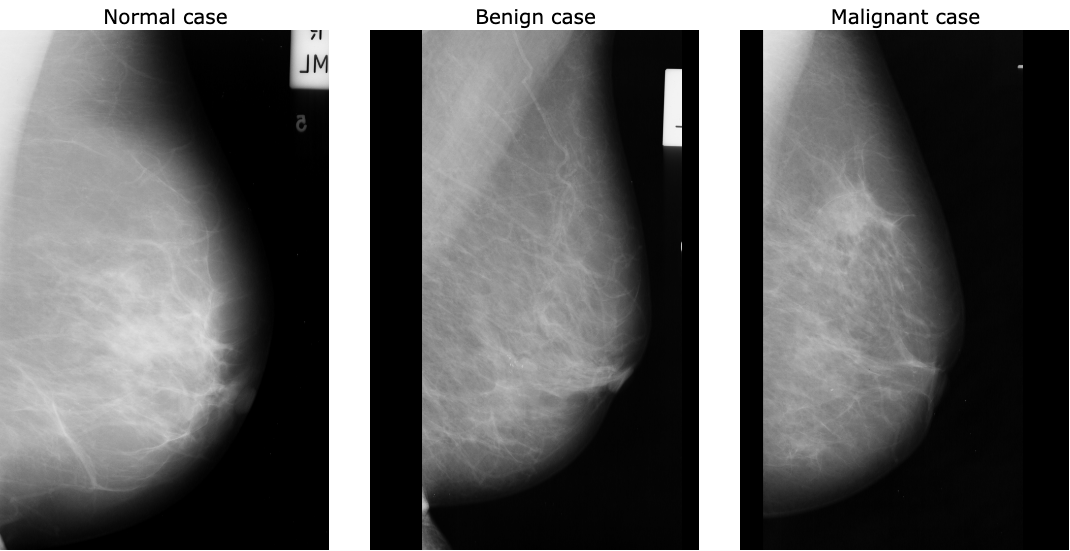
\includegraphics[width=\textwidth]{Dissertation/figures/introduction/mammogram examples.png}}
\caption{\label{fig:introduction-mammogram-examples}Example of three types of mammograms, including normal, benign and malignant cases. Figures extracted from the mini-MIAS dataset (Suckling, 1994). Created using draw.io.}
\end{figure}

Indeed, error-prone mammogram interpretations by radiologists can lead to decisions that can ultimately harm the patients. On one hand, breast cancers can be missed altogether, inducing an absence of treatments for sick patients, while on the other hand, an instance of breast cancer can be reported when in reality there is no cancerous tumour, leading to unnecessary treatment being carried out \citep{Elter2009}. To that end, using Computer-Assisted Detection (CAD) software can help minimise the number of wrong interpretations and increase the accuracy of mammography screening \citep{Shen2017}.\\

The motivation behind this project is to implement a system to accurately detect breast cancer in order to prevent late treatments due to false negatives as well as preventing unnecessary treatments in cases of false positives. Ultimately, the long-term target of this project is to combine it with other deep learning algorithms developed across other projects supervised by Dr David Harris-Birtill (past and present). This will allow a general artificial intelligence system capable of detecting multiple forms of cancer with higher accuracies than radiologist diagnostics.\\

%%%%%%%%%%%%%%%%%%%%%%%%%%%%%%%%%%%%%%%%%%%%%%%%%%%%%%%%%%%%%%%%%%%%%%%%%%%%%%%%%%

\section{Problem Description}
\label{sec:problem-description}

CAD systems using deep learning techniques could in theory highly increase the accuracy of mammogram screenings for detecting early signs of breast cancers. However, these techniques require large amounts of data to learn its underlying patterns and adapt to new cases, powerful computing resources to accelerate the processing of learning the data, and are often very hard to optimise and .\\

Parts of the work undertaken during this project will be conducted as a group comprised of two other members, Ashay Patel and Shuen-Jen Chen. Section~\ref{sec:introduction-objectives} covers in more detail which tasks will be conducted personally and in a group. The reasoning behind these common tasks is for a functional pipeline to be reached earlier, eventually allowing each group member to further explore deep learning techniques individually more quickly due to the limited time frame of this project, using the common basic pipeline as a starting point.

%%%%%%%%%%%%%%%%%%%%%%%%%%%%%%%%%%%%%%%%%%%%%%%%%%%%%%%%%%%%%%%%%%%%%%%%%%%%%%%%%%

\section{Objectives}
\label{sec:introduction-objectives}

The main objective of this project consists of implementing a deep learning pipeline that will be able to learn how to detect cases of breast cancer in mammograms. This objective is broken down into two steps:
\begin{itemize}
    \item \textbf{Group work}: a common deep learning pipeline will be initially implemented as part of a group with Ashay Patel and Shuen-Jen Chen over the course of a three-week period, including data cleaning and pre-processing, results output and a basic deep learning model. The distribution of tasks between the group can be found in Appendix~\ref{ch:appendix-team-meeting-summaries}.
    \item \textbf{Individual work}: the aforementioned pipeline will then be individually extended by introducing techniques that differ from the ones found in existing literature.
\end{itemize}

To reach this goal, an extensive literature review has to first be written to cover the background of deep learning techniques applied to the field of cancer detection and to review existing results. These include identifying results achieved using different methods (e.g. traditional machine learning techniques) and reviewing state of the art deep learning techniques applied to the detection of breast cancer in mammograms. This step is primordial as it will guide the research towards the most promising areas, as well as govern the choice of techniques to implement and explore in further sections.\\

The final results achieved individually will finally be compared with the common deep learning pipeline designed in group, as well as the results gathered by the two other group members and the results found in papers that used similar approaches.

%%%%%%%%%%%%%%%%%%%%%%%%%%%%%%%%%%%%%%%%%%%%%%%%%%%%%%%%%%%%%%%%%%%%%%%%%%%%%%%%%%

\section{Report Structure}

\tab \textbf{Introduction} \space 
Presents an overview of the subject's background through the problem description and the motivation behind this project, followed by the objectives that project aims to achieve.\\

\textbf{Context Survey} \space
Explores the literature and background surrounding breast cancer detection techniques, starting from primitive cancer detection systems, followed by traditional machine learning methods, and ending with the deep learning techniques that have been used in recent times.\\

\textbf{Ethics \& Datasets} \space
Considers the ethical issues taken into account for this project and describes the datasets used.\\

\textbf{Design} \space
A high-level exploration of design considerations regarding the deep learning pipeline to implement and the software in general.\\

\textbf{Implementation} \space
Comprehensively covers the steps followed when implementing the deep learning pipeline, explaining the practical solutions to implement code. Additionally, covers any testing done to validate that the system works as expected.\\

\textbf{Evaluation} \space
A review of the different results to assess the efficiency of the different techniques used to train the and how it compares to other models, including the common pipeline, the other group member's results, and relevant results identified in the context survey.\\

\textbf{Conclusions} \space
A summary the accomplished project's objectives, its limitations, plans for future work, and a final reflection on the project as a whole.